%!TEX root = presentation.tex
\begin{frame}\frametitle{Overview}
	\only<1>{
		\begin{center}
			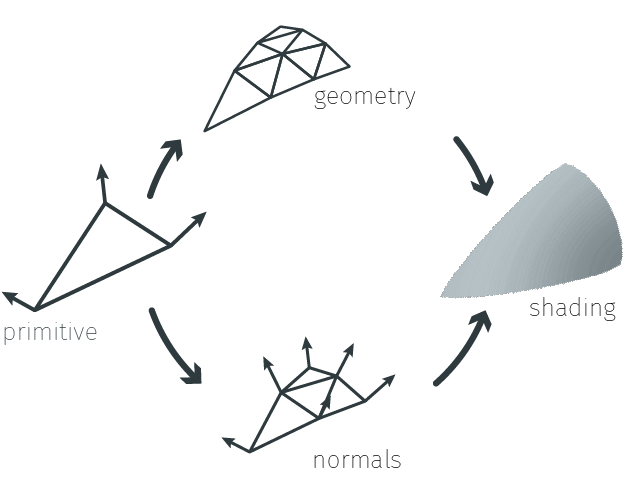
\includegraphics[width=\textwidth]{./img/1_single/recap_overview.png}
		\end{center}
	}
	\only<2>{
		\begin{center}
			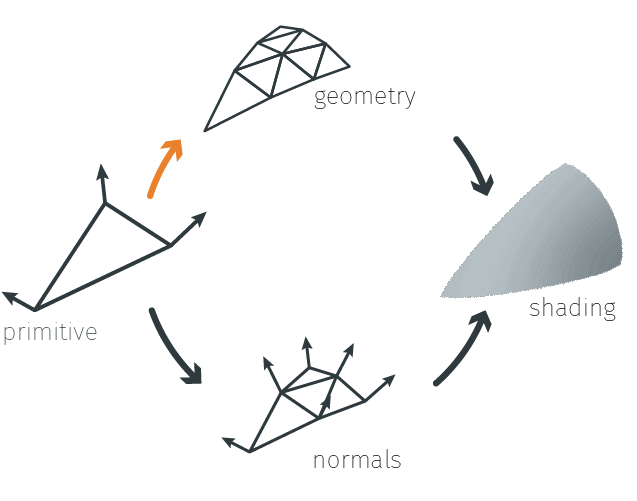
\includegraphics[width=\textwidth]{./img/1_single/recap_inputToGeom.png}
		\end{center}
	}
	\note<1>{\textbf{[Laura]} PN triangle is defined by geometry and normal component.}
	\note<2>{\textbf{Laura} From geometric component of input primitive to geometric component of PN triangle}
\end{frame}	

\begin{frame}\frametitle{Geometry}
	\enhancement{emphasize vertices better}
	\begin{columns}
		\begin{column}{0.6\textwidth}
			\begin{center}
				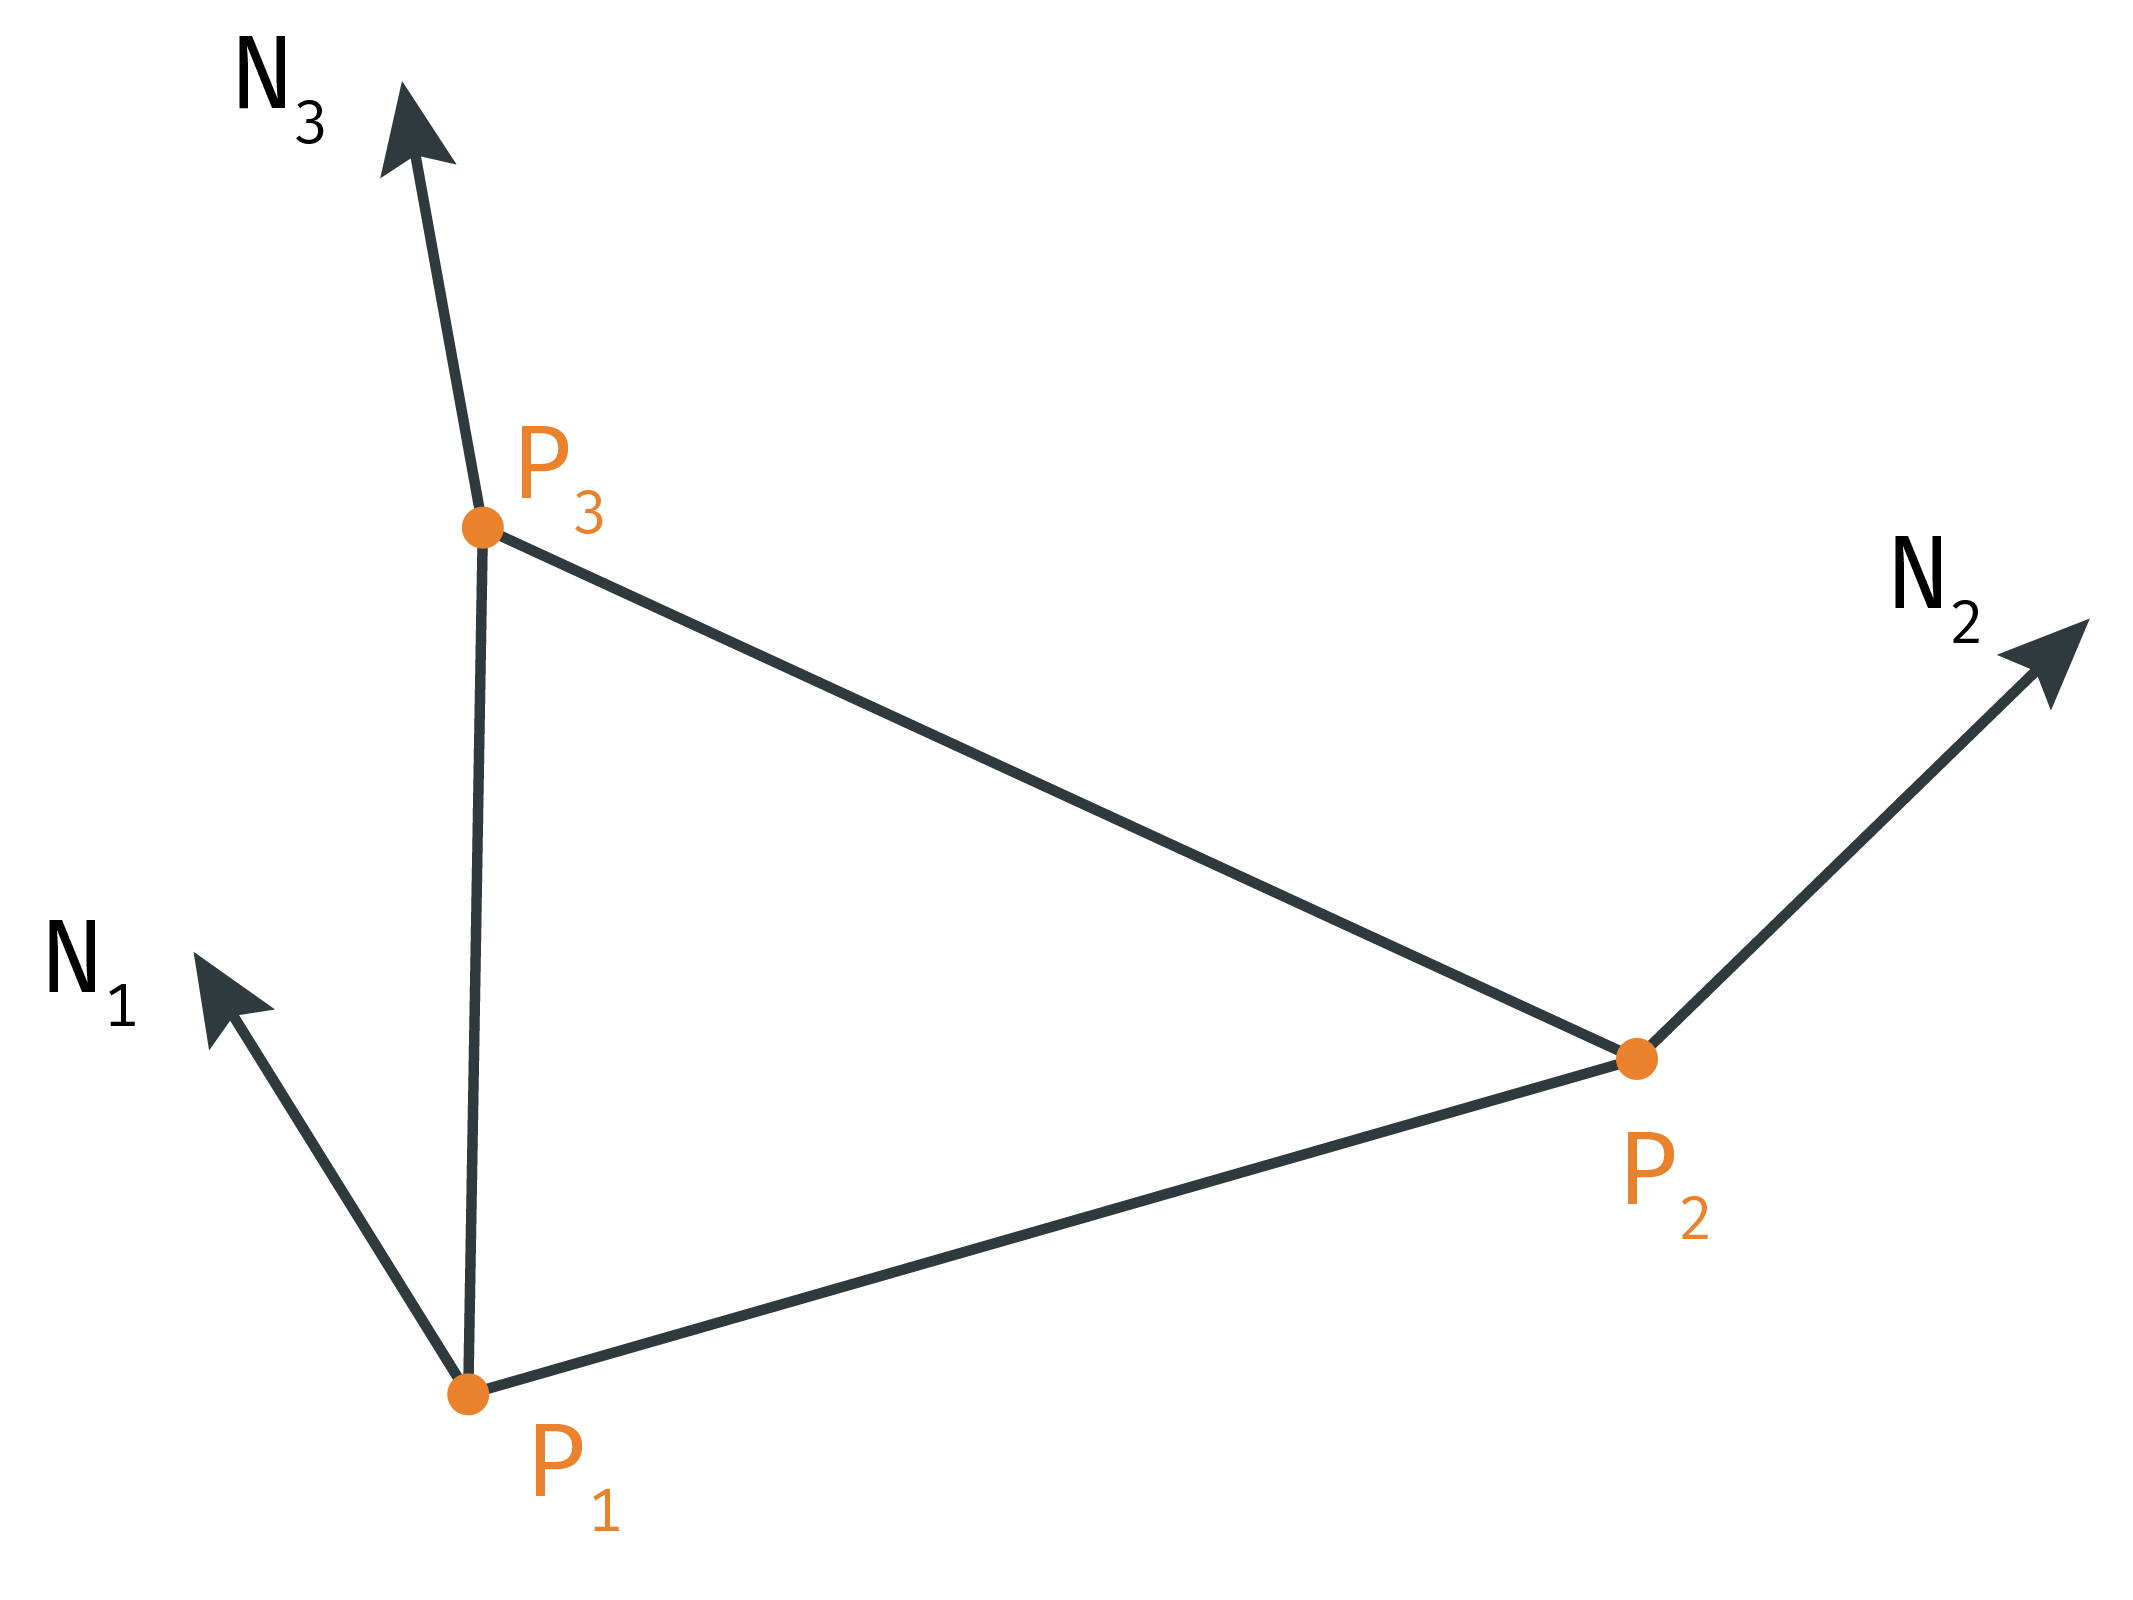
\includegraphics[width=\textwidth]{img/1_single/inputPrimitive_emphGeometry.png}
				\small{input primitive}
			\end{center}
		\end{column}
	\end{columns}
	\note{\textbf{[Laura]} This a standard triangle primitive, defined by its vertices and normals.\\ Focus on getting the different control primitives. \\
	Note that we only have this input primite, without information about its neighbours.}
\end{frame}

% Geometry process
\begin{frame}\frametitle{Geometry - Vertex Coefficients}
	\begin{columns}
		\begin{column}{0.6\textwidth}
			\begin{center}
				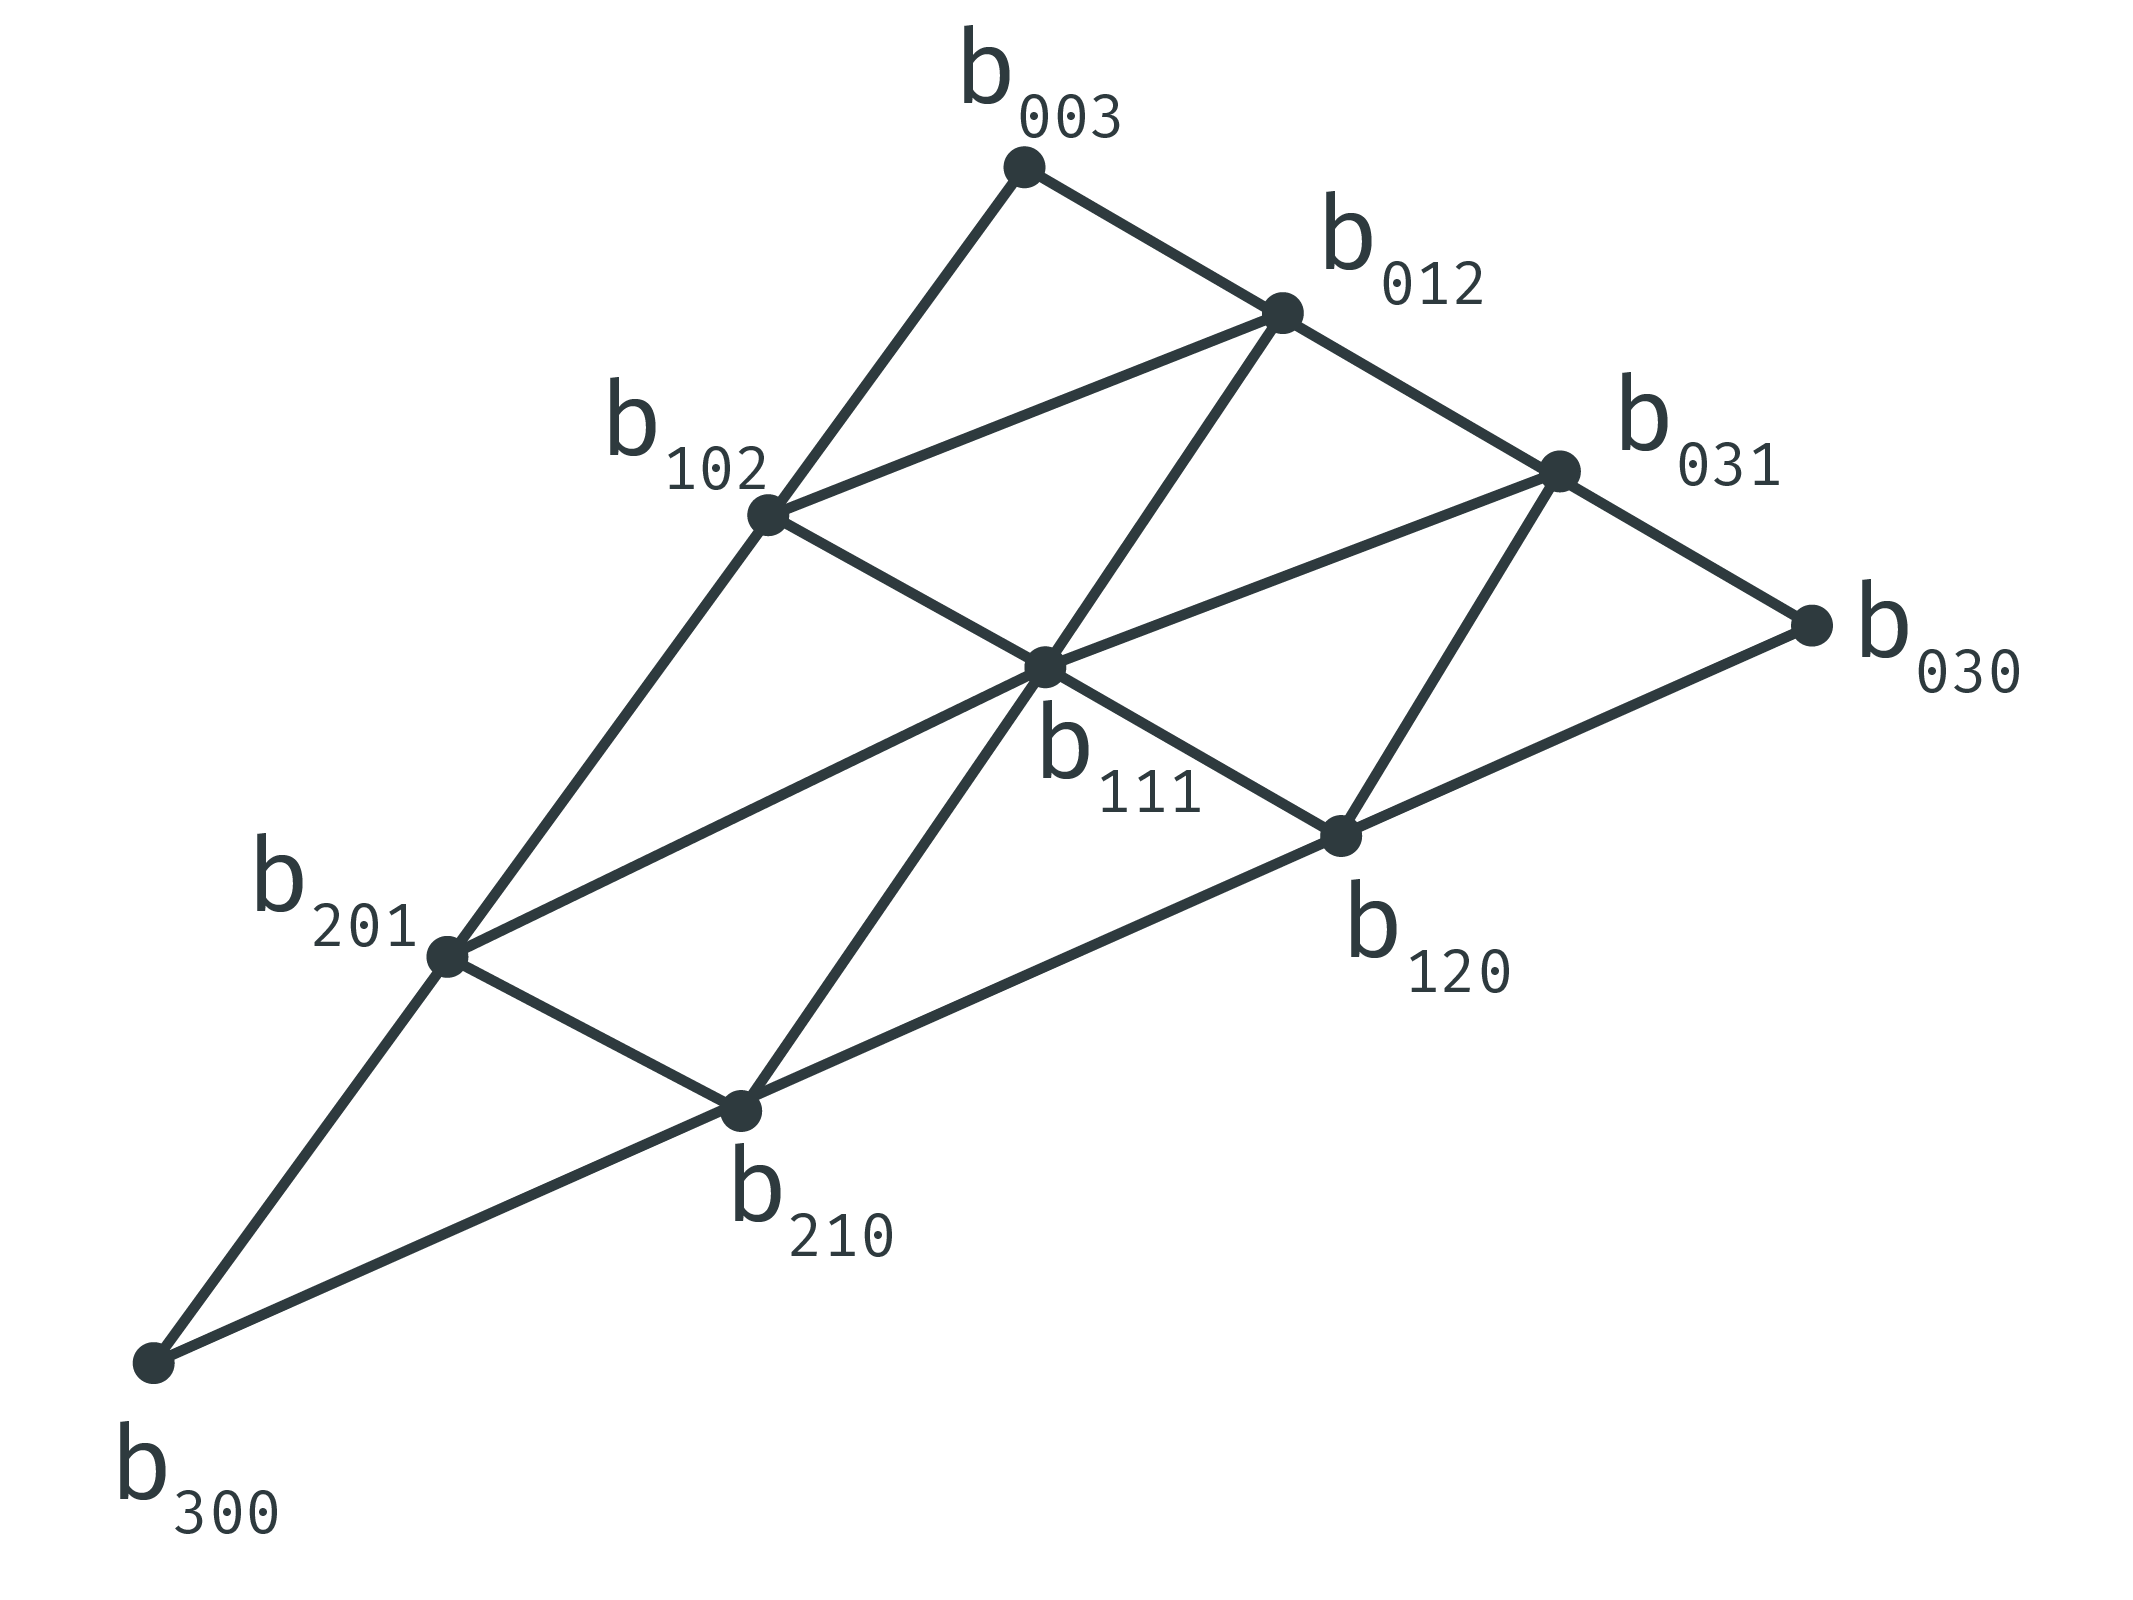
\includegraphics[width=\textwidth]{img/1_single/geometry_1.png}
				\small{control net}
			\end{center}
		\end{column}
			\begin{column}{0.4\textwidth}
				\uncover<2,3>{
				\begin{equation*}
					b_{ijk} = (iP_1 + jP_2 + kP_3)/3
				\end{equation*}
				}
				\uncover<3>{
				\begin{equation*}
					\begin{aligned}
					b_{300} & = P_1,\\
					b_{030} & = P_2,\\
					b_{003} & = P_3
					\end{aligned}
				\end{equation*}
				}
			\end{column}
	\end{columns}
	\note<1>{\textbf{[Laura]} These are all the initial control point. Evenly divided on the triangle. -> formula}
	\note<1>{\textbf{Laura} Mention which vertices are vertex, tangent and center coefficient.}
	\note<2>{\textbf{[Laura]} Nice formula}
	\note<3>{\textbf{[Laura]} Stress that the vertex coefficients/control points are the one on the original vertices and that they do not move.}
\end{frame}

\begin{frame}\frametitle{Geometry - Tangent Coefficients}
	\begin{columns}
		\begin{column}{0.6\textwidth}
			\begin{center}
			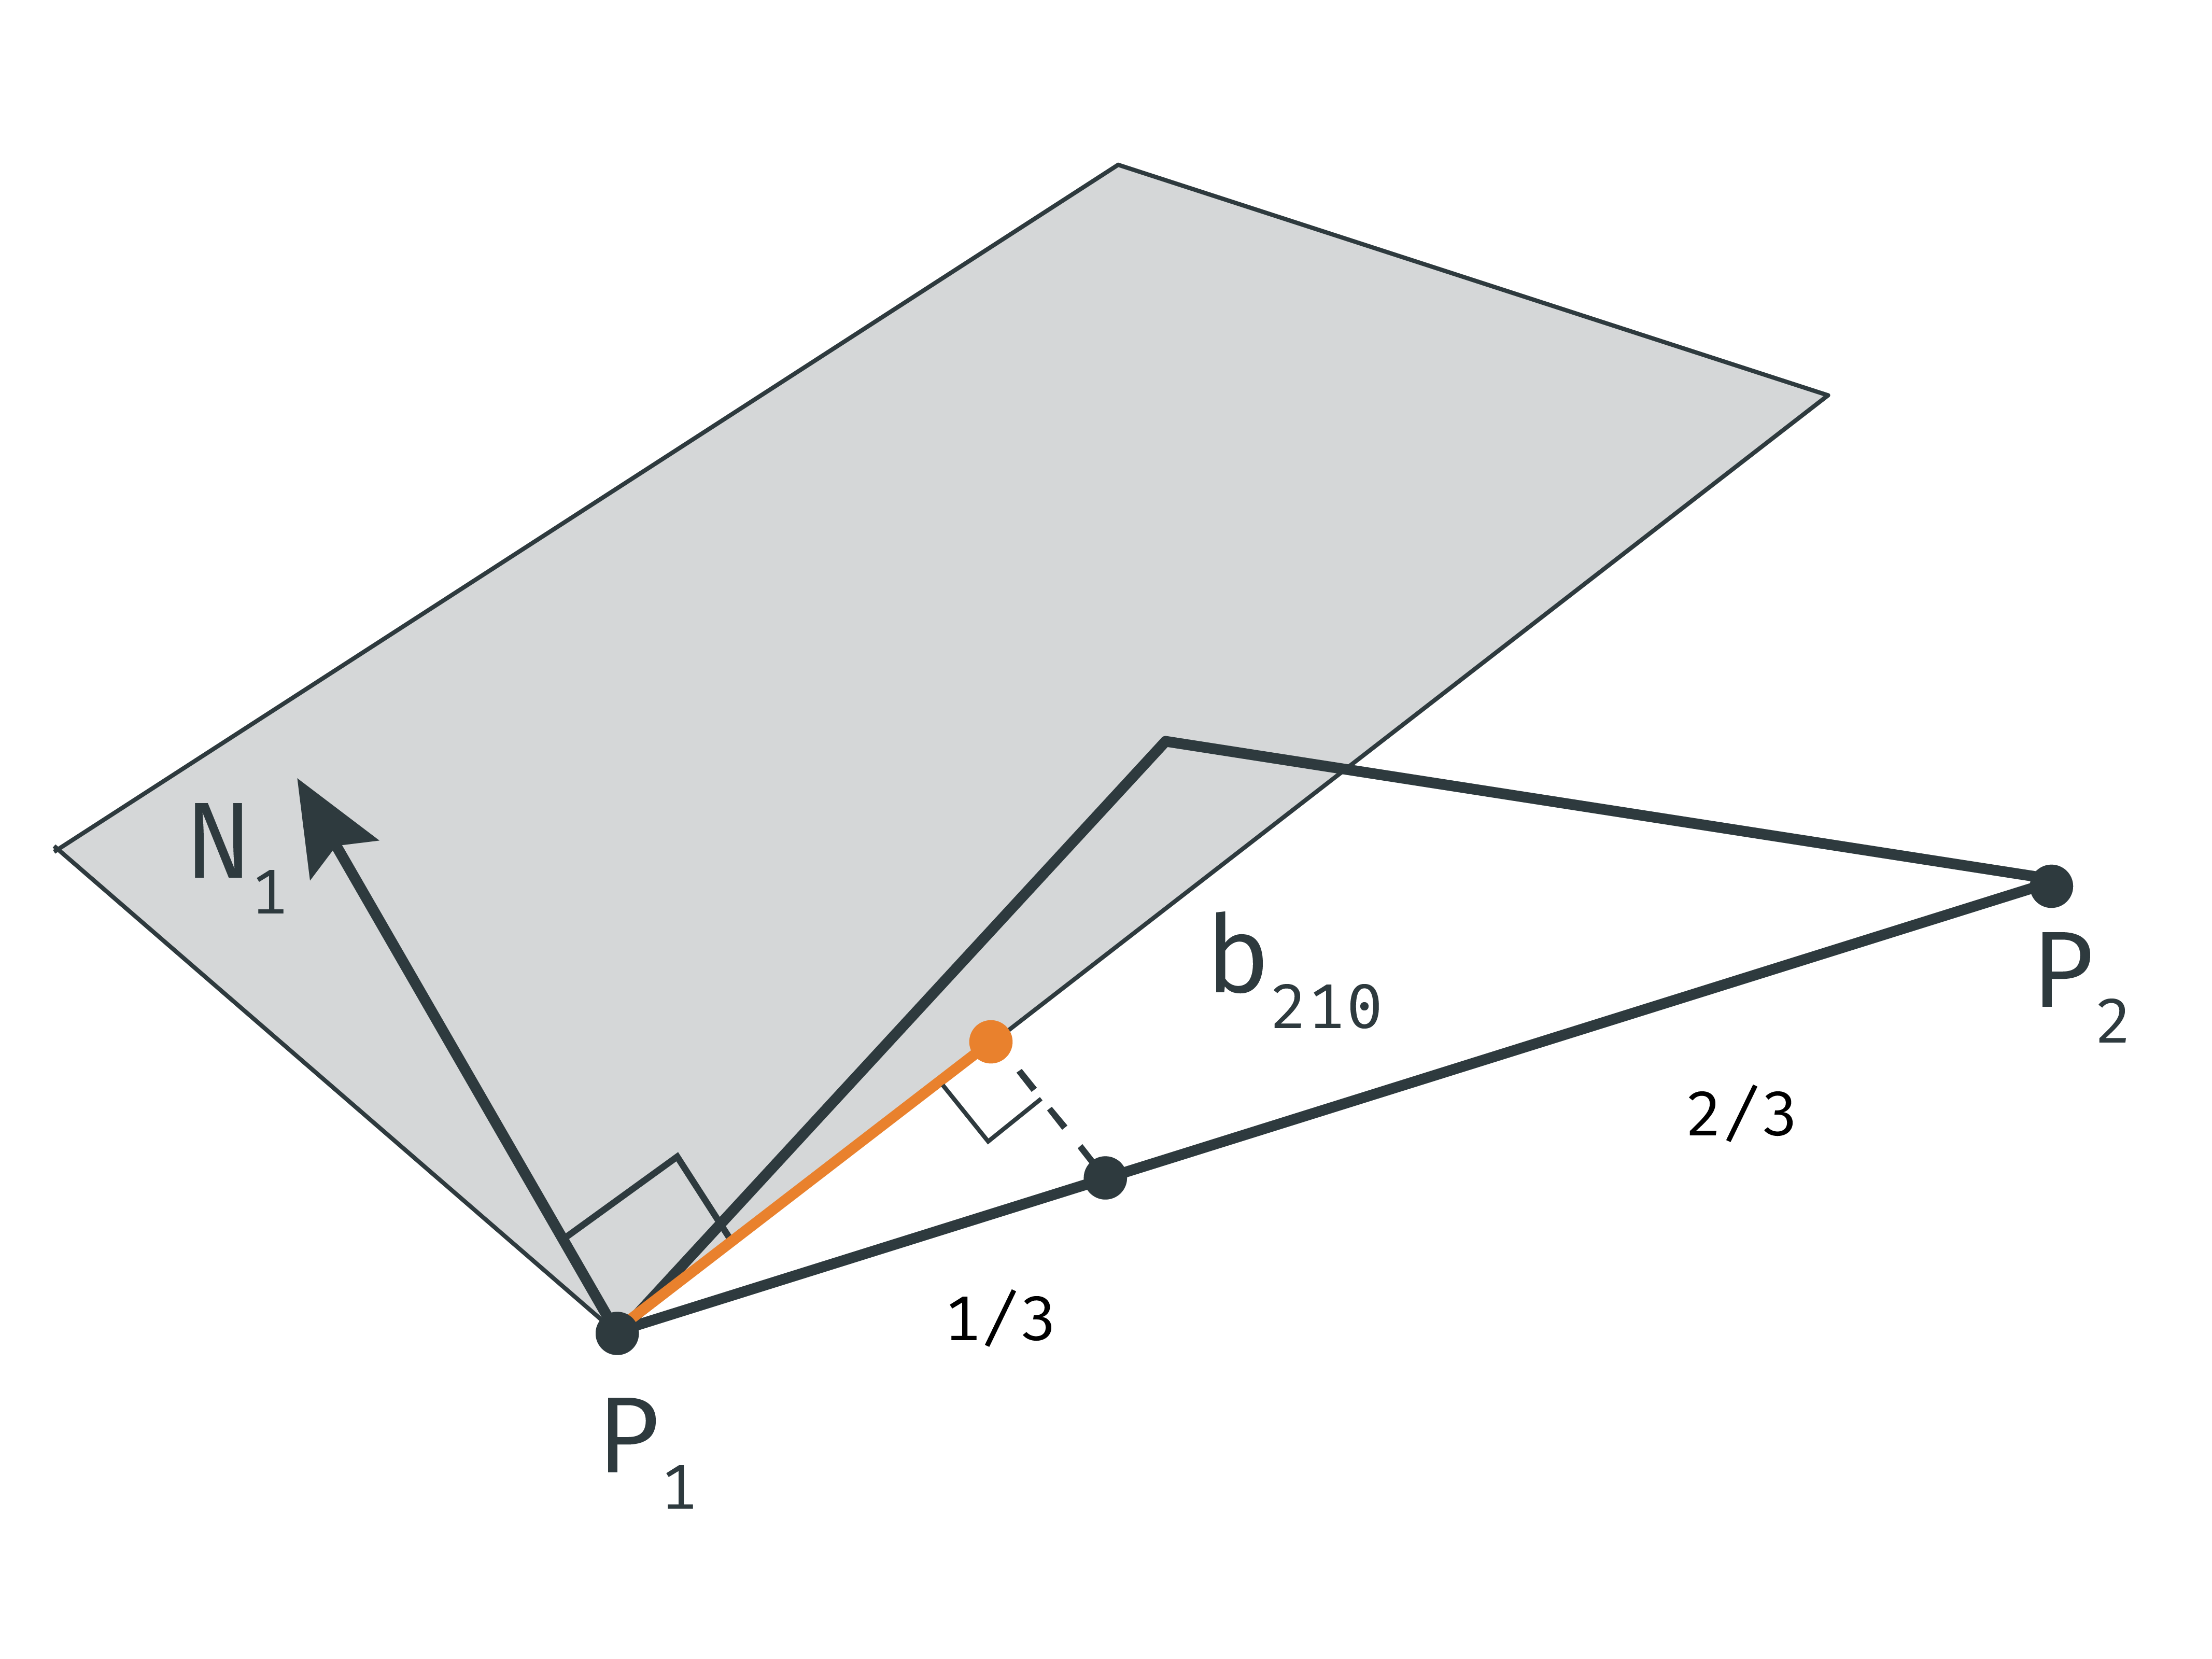
\includegraphics[width=\textwidth]{img/1_single/geometry_2.png}
			\small{normal projection}
			\end{center}
		\end{column}
		\uncover<2>{
			\begin{column}{0.4\textwidth}
				\begin{equation*}
					\begin{aligned}
					w_{ij} & = (P_j - P_i) \cdot N_i \in \mathbb{R} \\
					b_{210} & = \frac{2 P_1 + P_2 - w_{12}N_1}{3},\\
					~ & \vdots \\
					b_{201} & = \frac{2 P_1 + P_3 - w_{13}N_1}{3}
					\end{aligned}
				\end{equation*}
			\end{column}
		}
	\end{columns}
	\note{\textbf{[Laura]} Define a plane using the closest vertex and its normal. Find the point on this plane that is closest to the uniformly distributed point.}
\end{frame}

% b_{120} & = (2 P_2 + P_1 - w_{21}N2) / 3,\\
% b_{021} & = (2 P_2 + P_3 - w_{23}N2) / 3,\\
% b_{012} & = (2 P_3 + P_2 - w_{32}N3) / 3,\\
% b_{102} & = (2 P_3 + P_1 - w_{31}N3) / 3,\\

\begin{frame}\frametitle{Geometry - Center Coefficient}
	\begin{columns}
		\begin{column}{0.6\textwidth}
			\begin{center}
			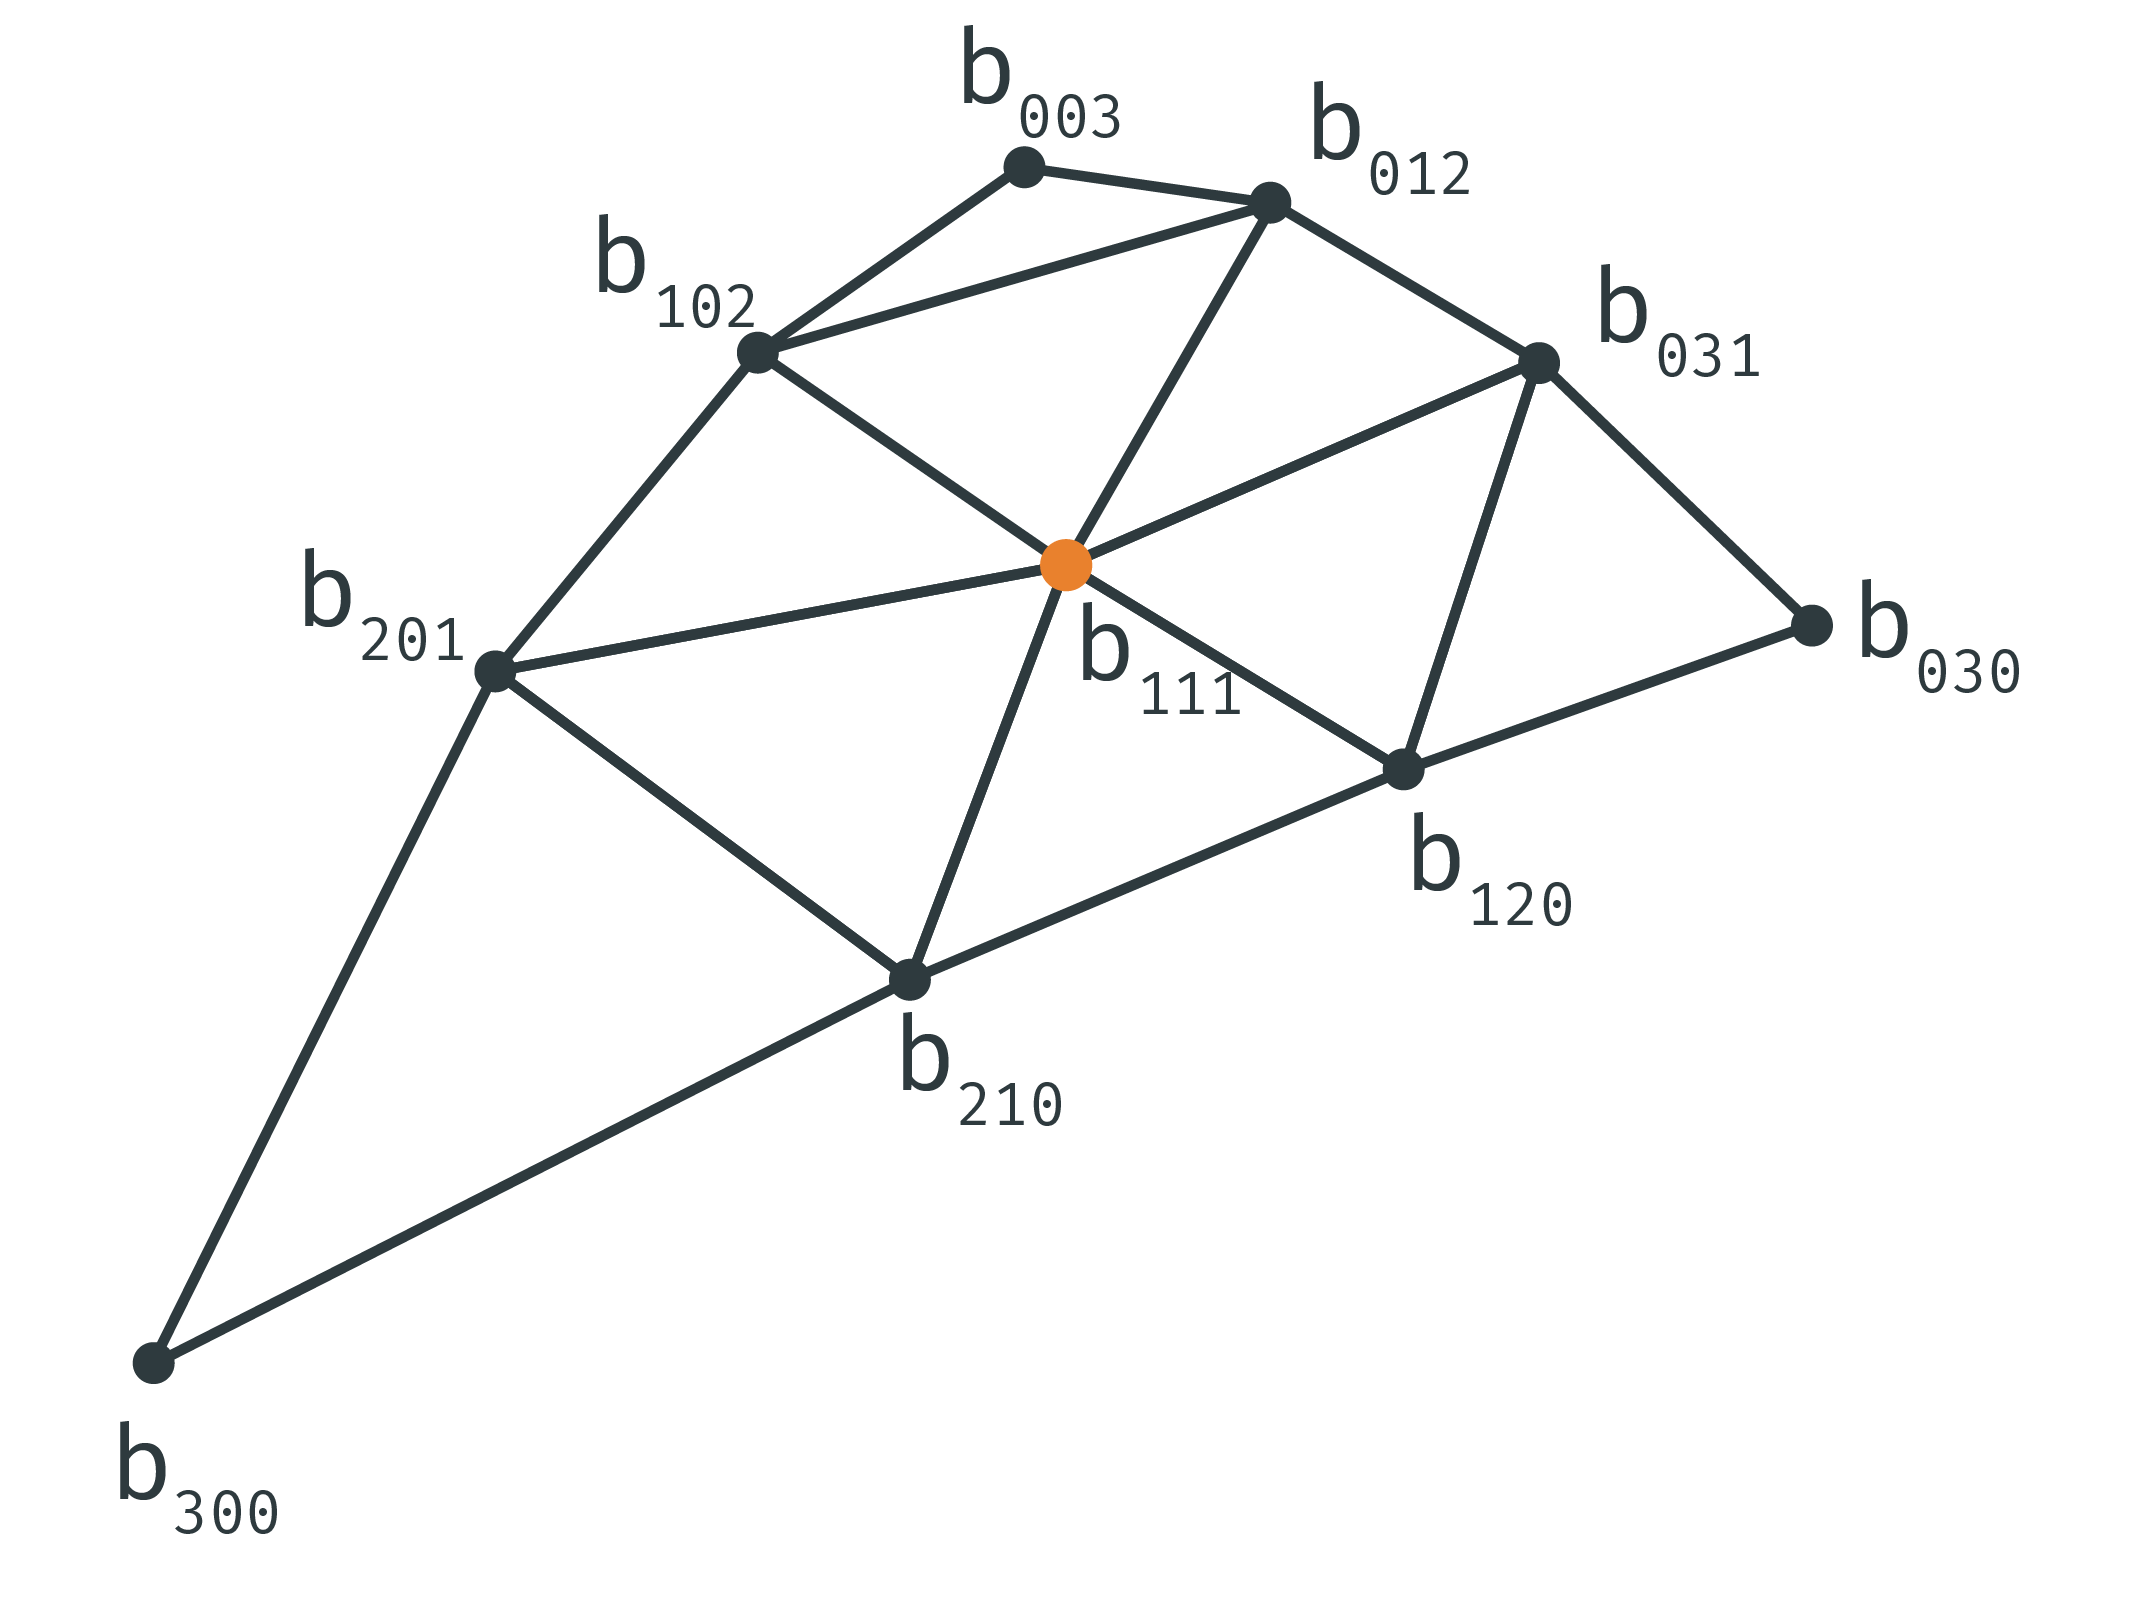
\includegraphics[width=\textwidth]{img/1_single/geometry_3.png}
			\small{center control point}
			\end{center}
		\end{column}
		\uncover<2>{
			\begin{column}{0.4\textwidth}	
				\begin{multline*}
				E = (b_{210} + b_{120} + b_{021} \\ 
				+ b_{012} + b_{102} + b_{201}) / 6,
				\end{multline*}
				\begin{equation*}
				\begin{aligned}
				V & = (P_1 + P_2 + P_3)/ 3, \\
				b_{111} & = E + (E - V) / 2
				\end{aligned}
				\end{equation*}
			\end{column}
		}
	\end{columns}
	\note<1>{\textbf{[Laura]} Note that this is the result of the previous step -> now only center coefficient is left.}
	\note<2>{\textbf{[Laura]} Average of the tangent coefficients plus  half the difference between the tangent and vertex coefficients.}
\end{frame}	

\begin{frame}\frametitle{Geometry - Result}
	\enhancement{Set result slide to plain}
	\begin{columns}
		\begin{column}{0.6\textwidth}
			\begin{center}
			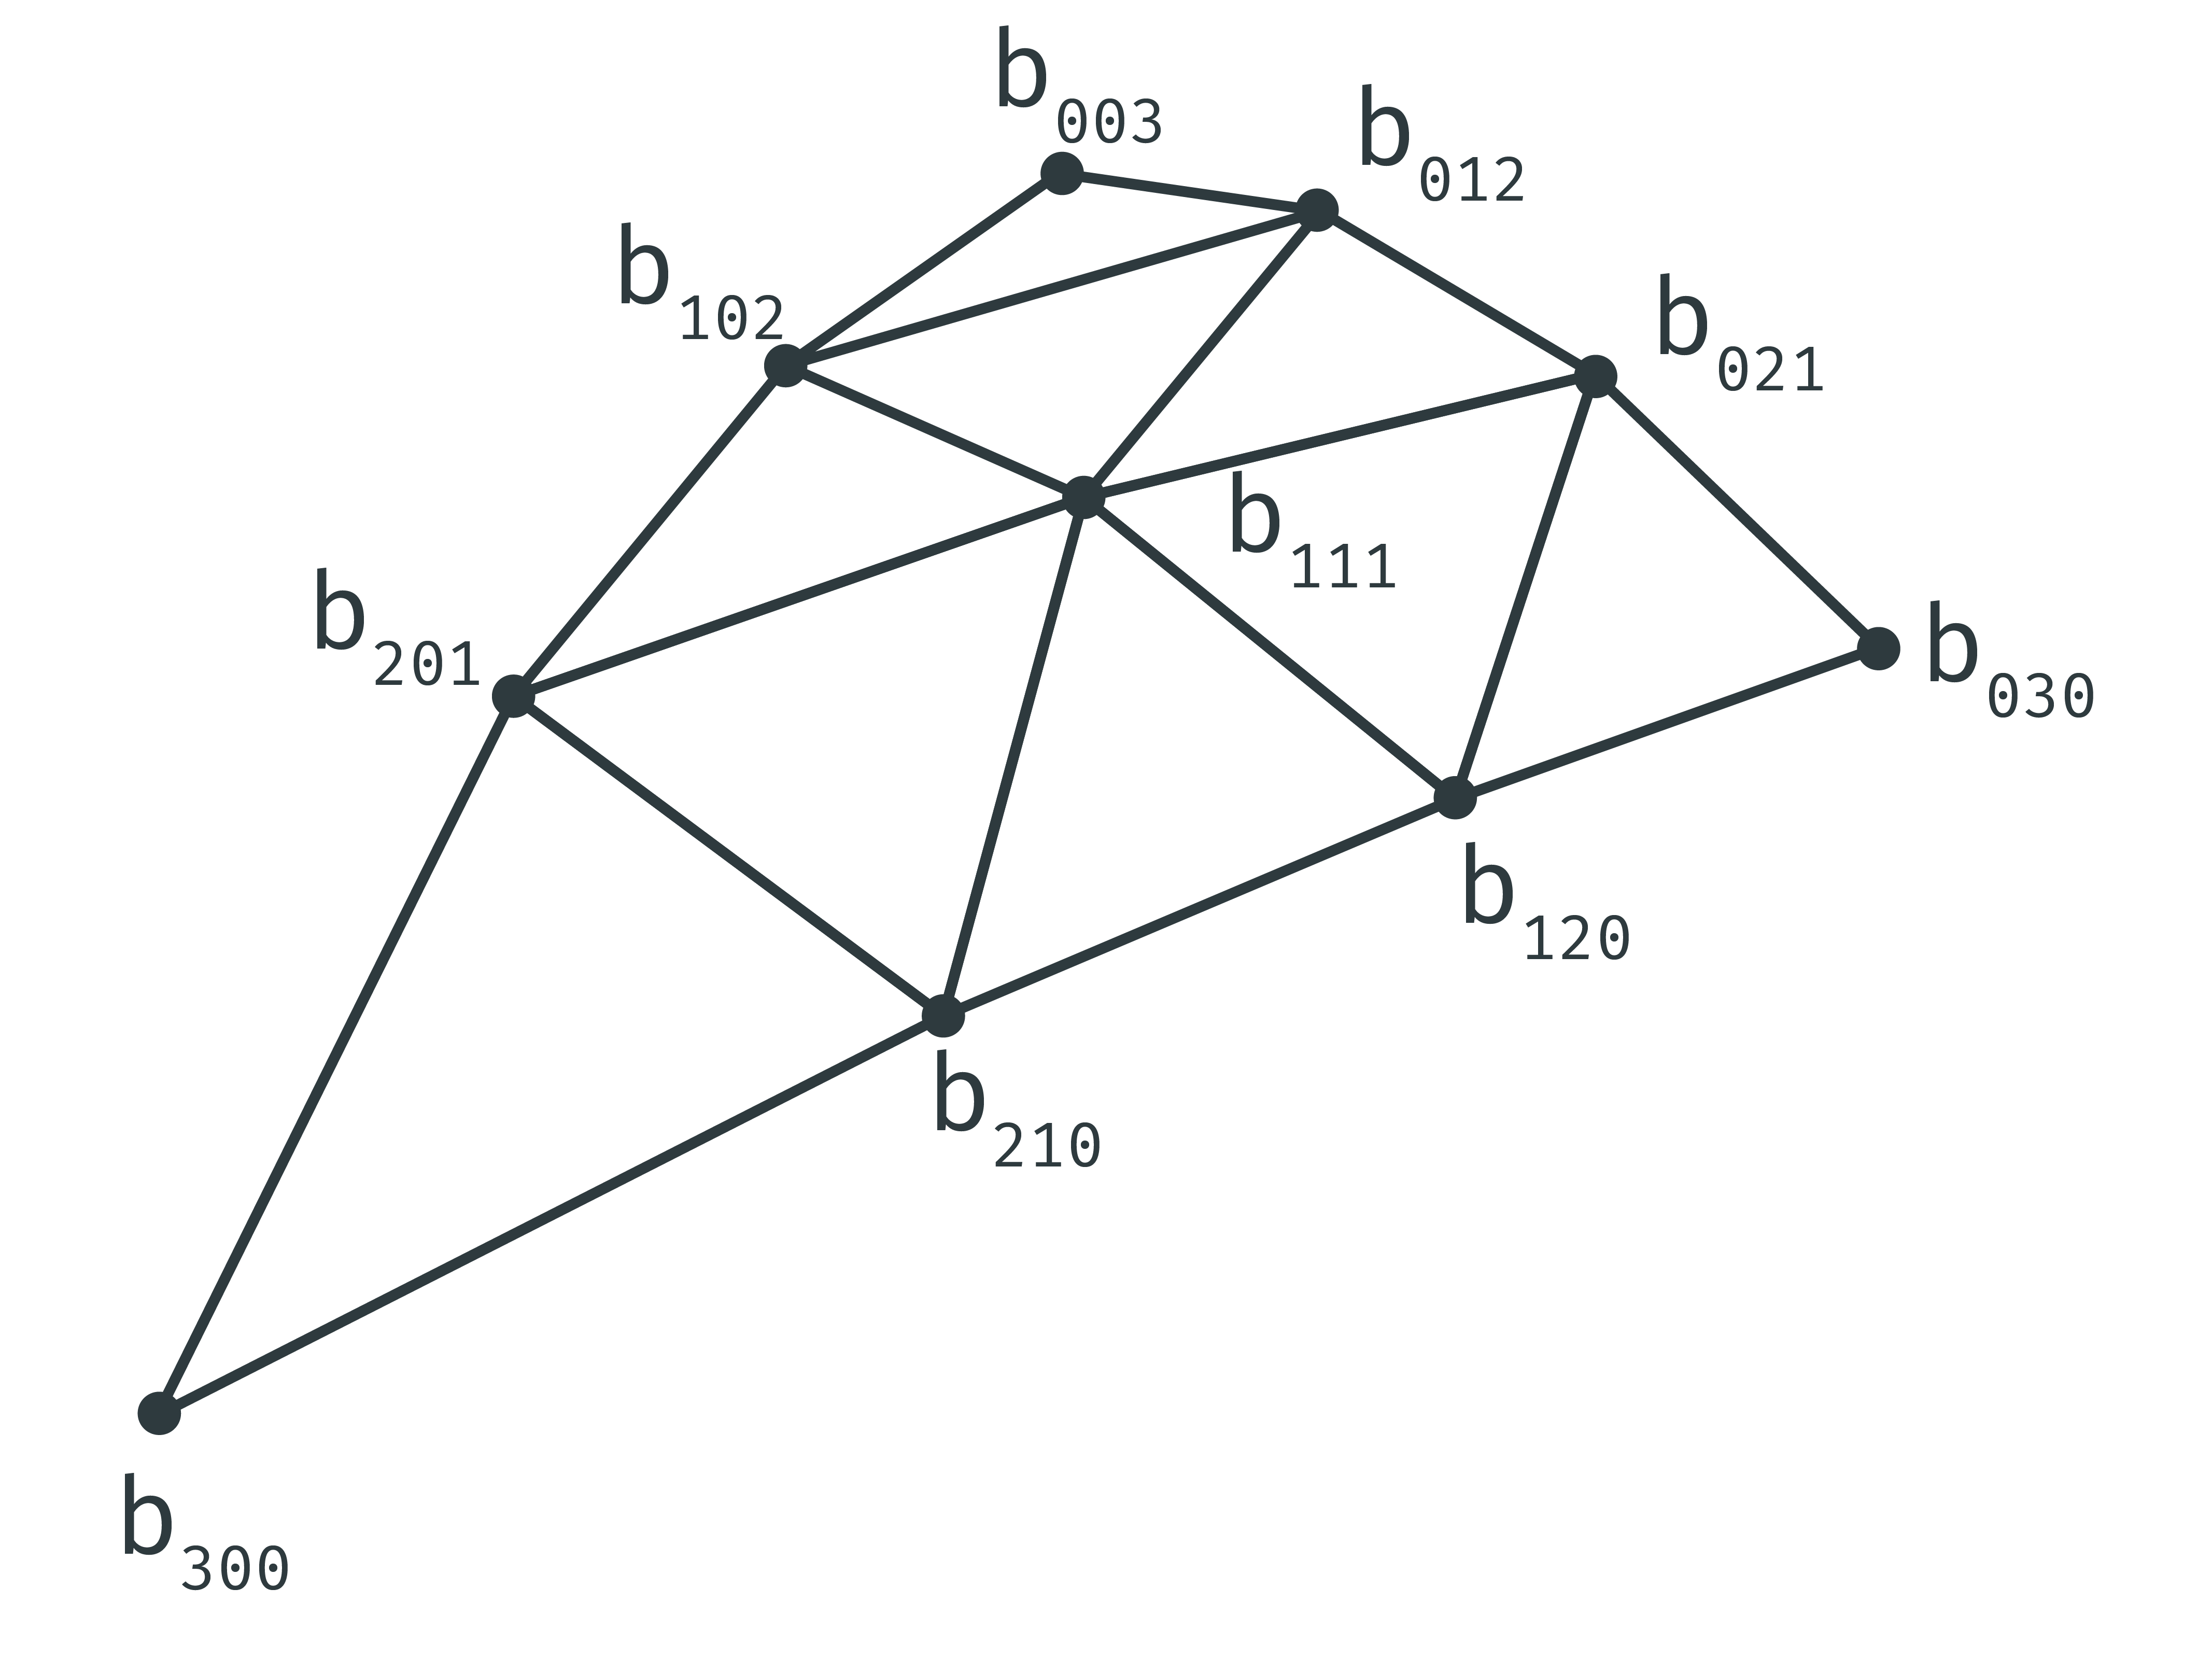
\includegraphics[width=\textwidth]{img/1_single/geometry_4.png}
			\end{center}	
		\end{column}
	\end{columns}
	\note<1>{\textbf{[Laura]} Results}
\end{frame}

\begin{frame}\frametitle{Overview}
	\begin{columns}
		\begin{column}{0.9\textwidth}
			\begin{center}
				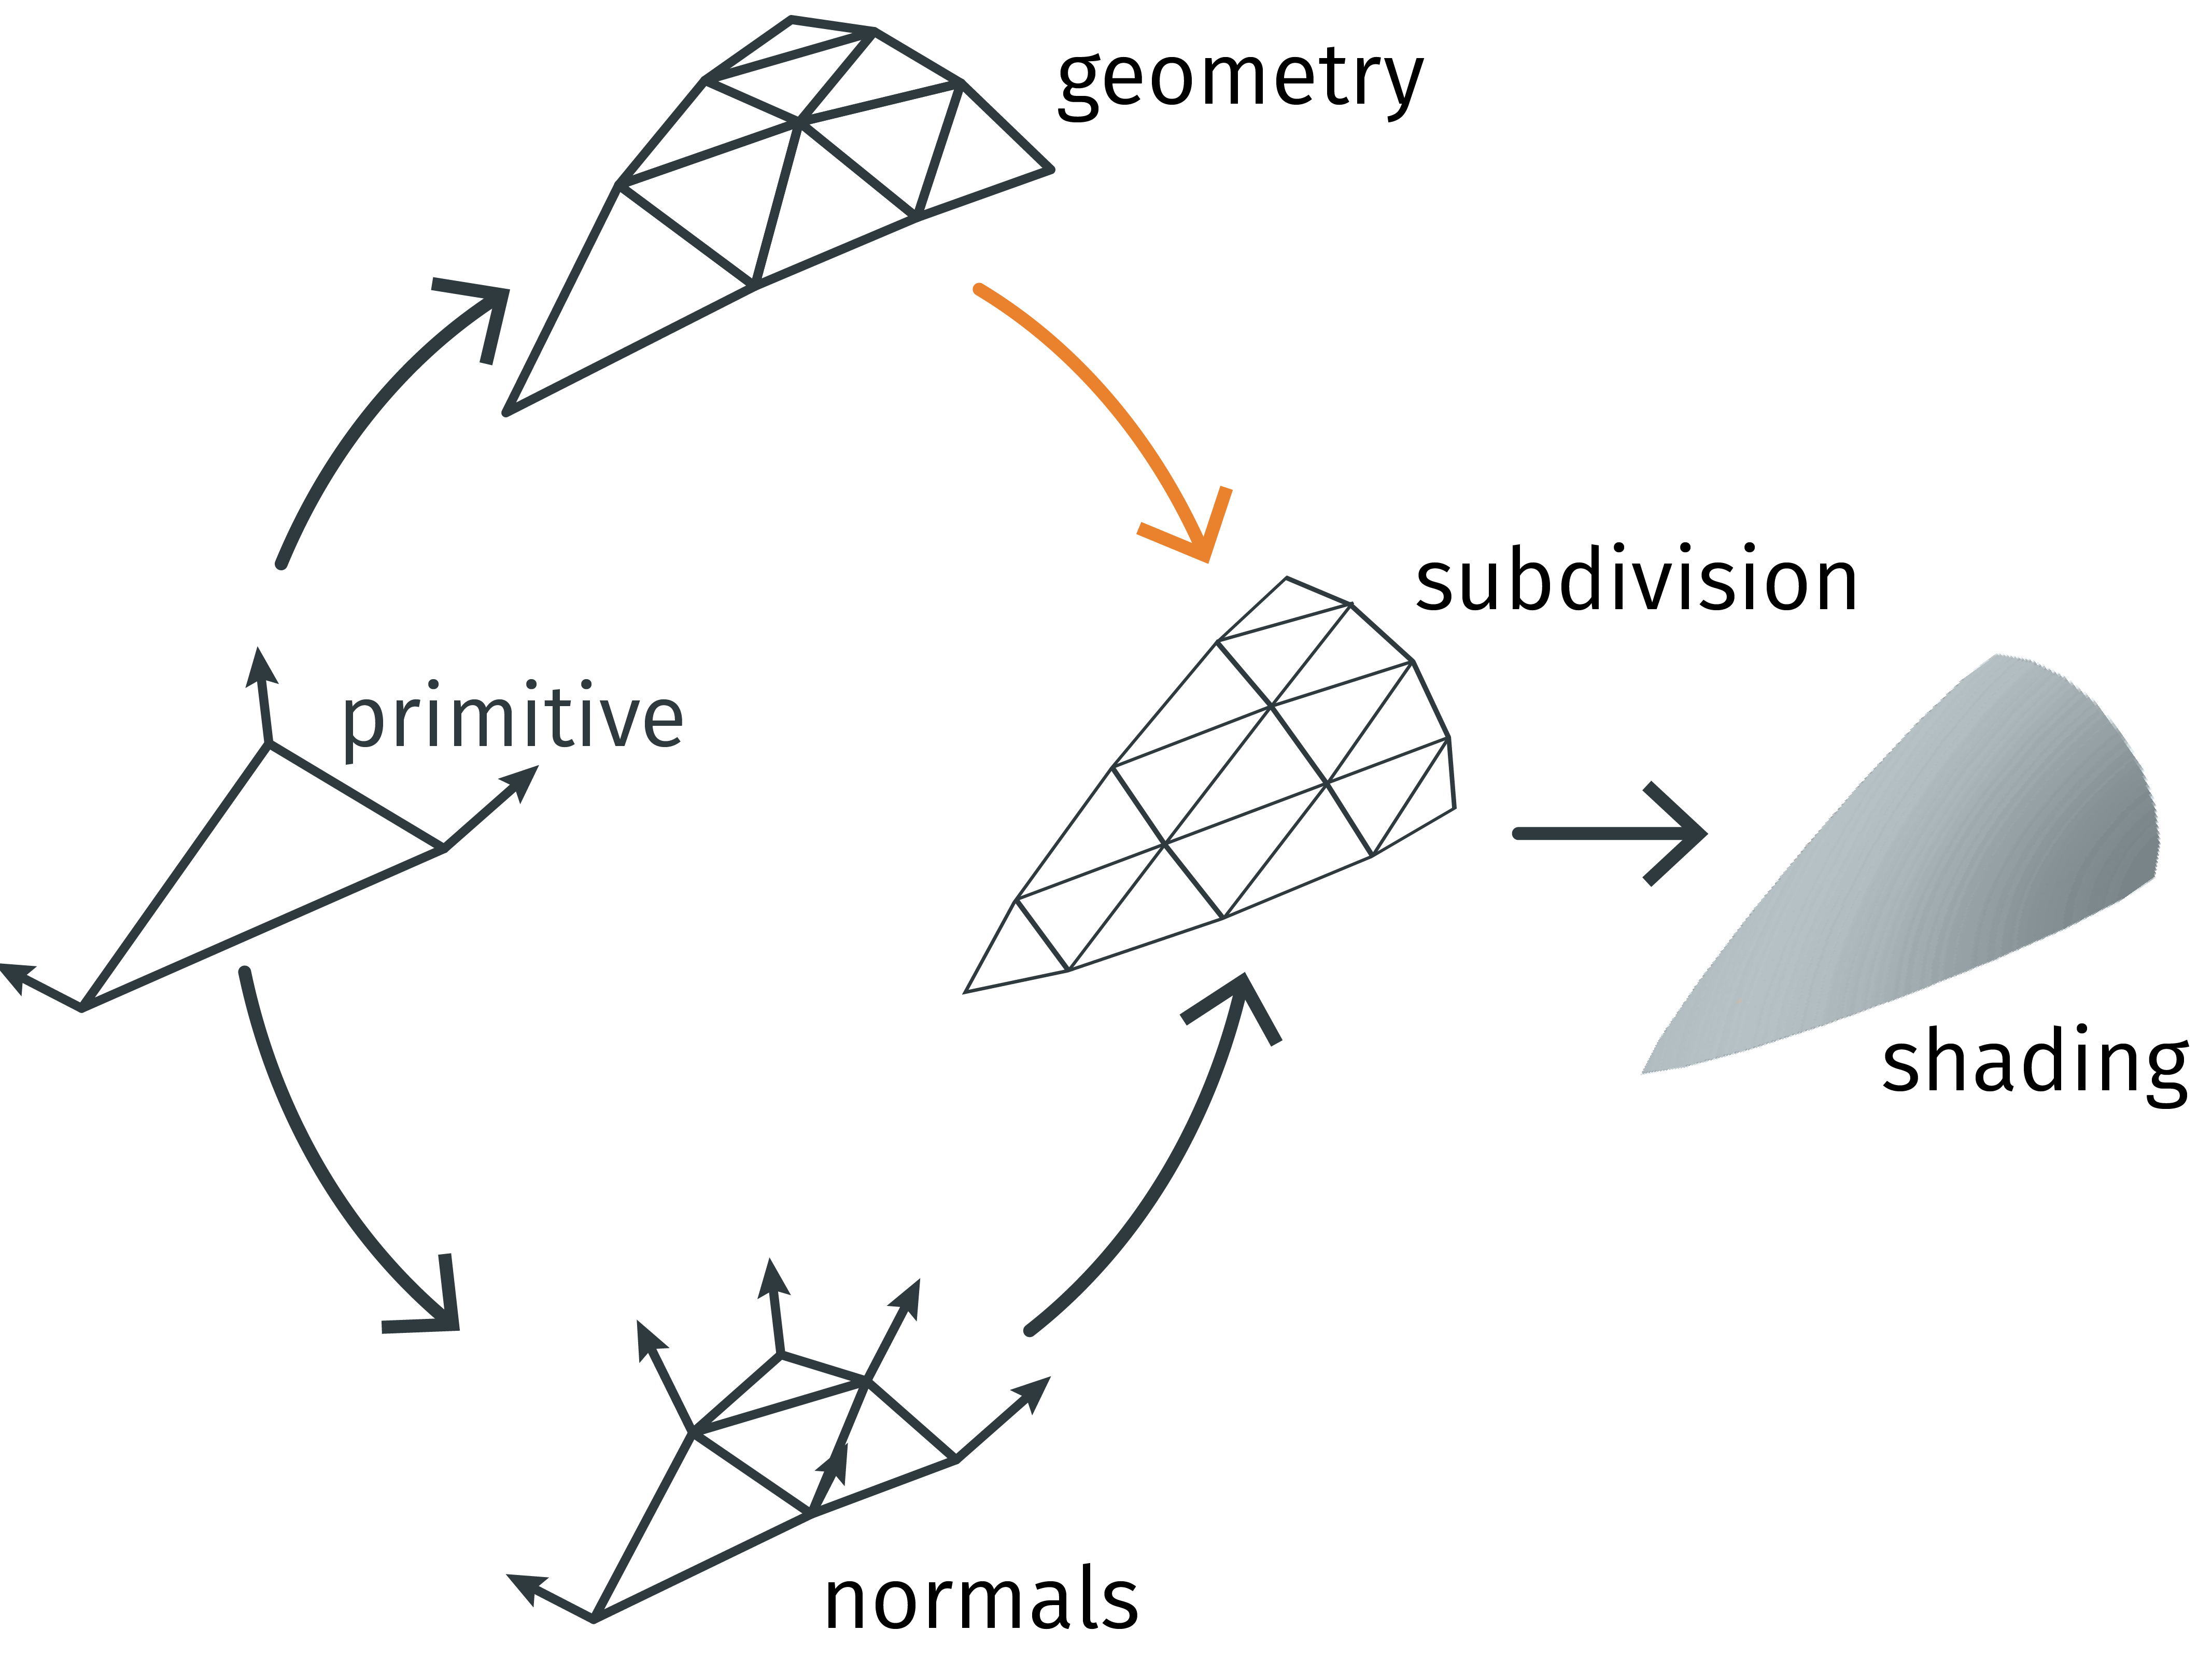
\includegraphics[width=\textwidth]{./img/1_single/recap_geomToShading.png}
			\end{center}		
		\end{column}
	\end{columns}
	\note<1>{\textbf{[Rick]} Overview -> how to get from this to shading. Sample/subdivide with formula on following slide.}
\end{frame}	

\begin{frame}\frametitle{Cubic B\'ezier patch}
	\begin{columns}
		\begin{column}{0.5\textwidth}
			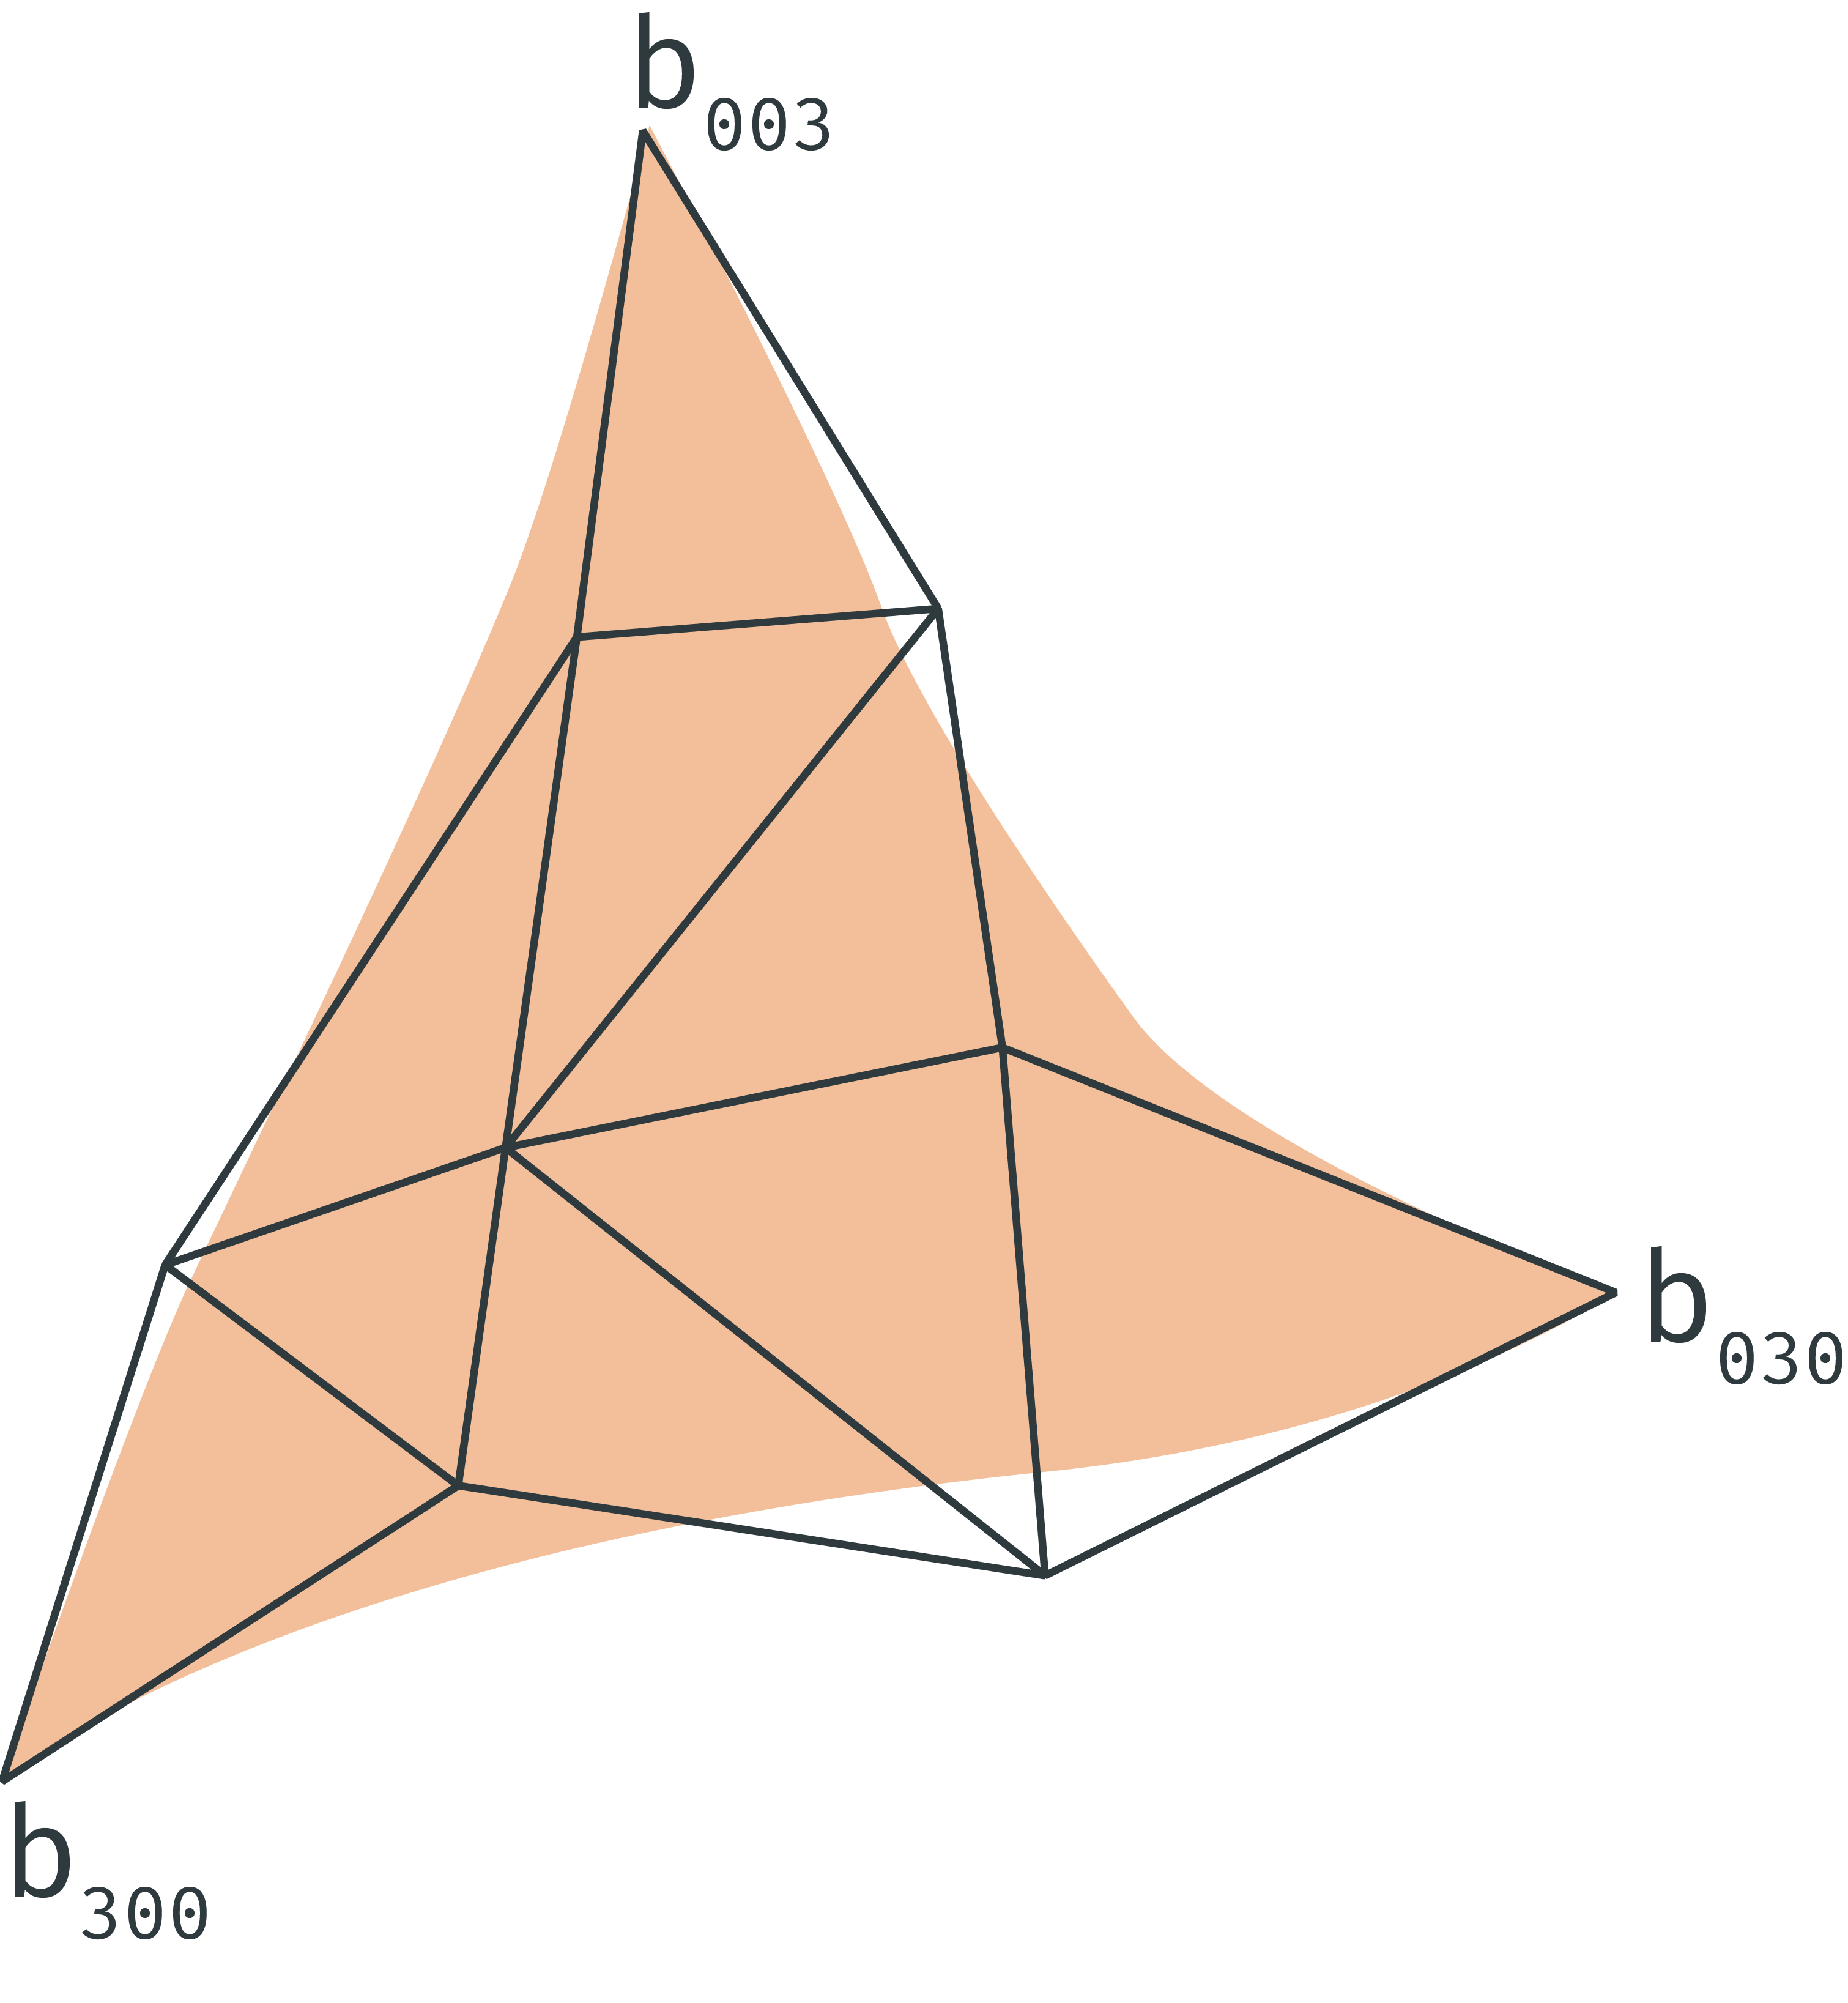
\includegraphics[width=\textwidth]{img/1_single/cubicPatch.png}
		\end{column}
		\begin{column}{0.5\textwidth}
			% \begin{equation*}
				% b: \mathbb{R}^2 \rightarrow \mathbb{R}^3 
				% \text{, for } w = 1 - u - v, u, v \text{, } w \geq 0
			% \end{equation*}
			\begin{equation*}
				w = 1 - u - v
			\end{equation*}
			\begin{equation*}
				u,\, v,\, w \geq 0
			\end{equation*}
			\begin{equation*}
				b(u,v) = \sum\limits_{i+j+k=3} b_{ijk} \frac{3!}{i!j!k!} u^i v^j w^k
				% & = b_{300} w^3 + b_{030} u^3 + b_{003} v^3 \\
				% & + b_{210} 3 w^2 u + b_{120} 3 w u^2 + b_{201} 3 w^2 v\\
				% & + b_{021} 3 u^2 v + b_{102} 3 w v^2 + b_{012} 3 u v^2\\
				% & + b_{111} 6 w u v.
			\end{equation*}
		\end{column}		
	\end{columns}
	\note<1>{\textbf{[Rick]} Very nice formula with a nice picture. Mention \textbf{Barycentric coordinates}}
	\note{u, v, w are a convex combination}
\end{frame}